\section{Results}
\label{SECIV}\label{sec:results}

In this section we test our implementation of the \lloid\ method using the
pipeline described in the previous section.  We answer the following questions
%
I) What is the measured loss of SNR due to the approximations used in the
\lloid\ algorithm in a realistic analysis pipeline?
%
II) What is the measured latency of the implementation described in section
\ref{sec:implementation}?
%
III) What is the measured computational cost of the implementation described in
section \ref{sec:implementation}?

\subsection{Measured \SNR\ loss}

We expect two contributions to the \SNR\ loss to arise in our implementation of
the \lloid\ algorithm.  The first is the \SNR\ loss due to the truncation of
the SVD basis, which is fundamental, and estimates for it
exist~\cite{Cannon:2010p10398}.  The second comes from non ideal
implementations of resampling that cause signal loss.  We have measured the
effect of the resampling in the pipeline alone on a single waveform to gauge
the magnitude of the loss.  It is shown in figure \ref{fig:resamp_mm} as a
function of the quality of the {\tt audioresample} element (which is
proportional to the filter length used).  In both cases we have to compare the
\SNR\ loss to the expected \SNR\ loss that arises from the discreteness of the
template bank which is typically $\sim 3\%$.  We will consider a comparable
\SNR\ loss to be tolerable, but ideally would like to have a factor of 10 lower
loss from the \lloid\ implementation (i.e. no more than $\sim 0.3 \%$).  
%
\begin{figure}
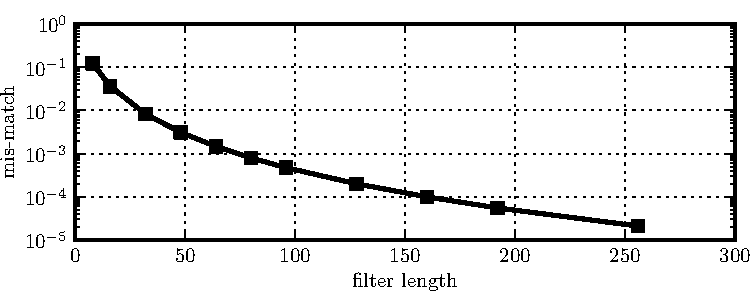
\includegraphics{resamp_mm.pdf}
\caption{\label{fig:resamp_mm}Mis-match as a function of the {\tt
audioresample} element's quality parameter.  Increasing the quality changes the
length of the sinc function filter that is used to decimate and interpolate the
data and filter output in our test pipeline.  Choosing a quality of 4
corresponds to a filter length of 64 samples and results in an acceptable loss
of .2 \% in \SNR\ for the chosen waveform.}
\end{figure}



\subsection{Measured latency}

\subsection{Measured computational cost}

%\FIXME{
%I would like to see this section changed to emphasize the low-latency time
%domain filtering 1. Use a live simulated white noise source (this ignores the
%latency of whitening, but that goes beyond the scope of this paper, and we
%mention this and perhaps suggest some exporation 2. Use TD filtering of N
%templates 3. Present the performance and latency and provide estimates for
%number of cores required for realtime ALIGO search based on current
%infrastructure 4. Compute the impulse responses of the templates and histogram
%the SNR loss for the SVD and time/slice/resampling 5. Put  a tee after some of
%the low frequency stages and perhaps test the possibility of predictive
%filtering (also with latency measurments) This will remove the complications of
%running a full pipeline.  We need to sort things out before we do that, and
%this paper should not be delayed any further.  The above tests will make the
%point we need to make
%}

%\subsection{Detector noise characteristics}

%We tested the new detection method with mock Advanced \textsc{ligo} data having a power spectrum prescribed by the ``zero detuning, high power'' noise model in \cite{Shoemaker:2009p9770}.
